\documentclass[12pt]{article}
\usepackage{amsmath, amsthm, amsfonts, graphicx}

\usepackage{euler}
\title{Abstract Algebra: Homework \#5}
\author{Joel Savitz}
\date{Wednesday 24 June 2020}

\newcommand{\reals}{\mathbb{R}}
\newcommand{\rats}{\mathbb{Q}}
\newcommand{\ints}{\mathbb{Z}}
\newcommand{\gltwo}{GL_2(\reals)}
\newcommand{\glmatrix}[4]{\ensuremath{\begin{bmatrix} #1 & #2 \\ #3 & #4 \end{bmatrix}}}
\newcommand{\glxmatrix}[9]{\ensuremath{\begin{bmatrix} #1 & #2 & #3 \\
#4 & #5 & #6 \\ #7 & #8 & #9 \end{bmatrix}}}
\newcommand{\glinverse}[4]{\ensuremath{\frac{1}{#1 #4 - #2 #3}\glmatrix{#4}{-#2}{-#3}{#1}}}
\newcommand{\ord}{\operatorname{ord}}
\newcommand{\freals}{\mathcal{F}(\reals)}
\newtheorem{thm}{Theorem}
\newtheorem{cnt}{Counterexample}

\begin{document}
\maketitle

\section{Chapter 11, Exercise A2}

Suppose $f = \binom{1\ 2\ 3\ 4\ 5\ 6}{6\ 1\ 3\ 4\ 5\ 4}$.

Then, $f$ generates a subgroup $S_6$
--- denoted $\langle f \rangle$ ---
like so:

\begin{align}
	f = & \binom{1\ 2\ 3\ 4\ 5\ 6}{6\ 1\ 3\ 2\ 5\ 4} \\
	f^2 = & \binom{1\ 2\ 3\ 4\ 5\ 6}{4\ 6\ 3\ 1\ 5\ 2} \\
	f^3 = & \binom{1\ 2\ 3\ 4\ 5\ 6}{2\ 4\ 3\ 6\ 5\ 1} \\
	f^4 = & \binom{1\ 2\ 3\ 4\ 5\ 6}{1\ 2\ 3\ 4\ 5\ 6} = e \in S_6
\end{align}

\section{Chapter 11, Exercise B1}

Suppose we have some group $G$ such that
$\ord(G) = n$.

\begin{thm} \label{thm1}
	$G$ is cyclic $\iff \exists x \in G \ni \ord(x) = n$	
\end{thm}

\begin{proof}
	Since $G$ is cyclic,
	it must be generated
	by some element $a \in G$,
	and since $\ord(G) = n$,
	we can rewrite $G$ as
	$\{e, a, a^2, a^3, ..., a^{n-1} \}$.
	Then, since $a^n \in G$ and all other
	powers of $a$ are already present,
	we deduce that $a^n = e$,
	and therefore we have $\ord(a) = n$
	and we have the implication
	$G$ is cyclic $\implies \exists x \in G \ni \ord(x) = n$.

	Conversely,
	suppose we have some $a \in G$
	where $\ord(a) = n$.
	Then, by definition
	we have $a^n = e$.
	Define the following set $H$:
	$H = \{x \in G: a^{n-i} \ni 0 \le i < n \}$.
	First, note that $x \in H \implies x \in G$ by construction.
	We can see that $|H| = n$
	since every $a^{n-i}$ must be distinct
	due to the fact that $\ord(a)$ is defined
	to be the smallest positive integer
	where $a^n = e$.
	Then, since $|H| = n$ and every element is a power
	of $a$ under an operation closed on $G$,
	we must have that $x \in G \implies x \in H$
	and thus by the Axiom of Extentionality
	we have $H = G$.
	Then, $G$ is generated by some element $a \in G$
	so $G$ is cyclic.
	Thus, we have
	the implication that
	$\exists x \in G \ni \ord(x) = n \implies G$ is cyclic.

	Finally, since we have the implication in both directions,
	we must have the bidirectional implication
	$G$ is cyclic $\iff \exists x \in G \ni \ord(x) = n$.
	This proves theorem \ref{thm1}.
\end{proof}

\section{Chapter 11, Exercise B3}

Suppose $G$ is some group generated by $a \in G$
and suppose $b \in G$.

\begin{thm} \label{thm2}
	$\exists k \in \ints \ni k\ord(b) = \ord(a)$
	i.e. the order of $b$ is a factor of the order of $a$.
\end{thm}

\begin{proof}
	Let $n = \ord(a)$ and let $m = \ord(b)$.
	We have $m = \ord(b) \iff b^m = e$
	Since $G = \langle a \rangle$,
	we have $G = \{e, a, a^2, a^3, ..., a^{n-1} \}$.
	Since $b \in G$, we must have that
	$\exists z \in \ints \ni 0 < z \le n$
	such that $a^z = b$
	Then if we take both sides to the power of $m$
	we have $a^{mz} = b^m = e = a^n$.
	Then clearly $m$ is a factor of $n$
	Since $a^n = a^{mz}$,
	we must have an integer $k$ where
	$kmz = n$,
	therefore $m$ is a factor of $n$
	and the order of $b$ is a factor of the order of $a$.
\end{proof}

\section{Chapter 11, Exercise D1}

Suppose $G$ is a group and $a,b \in G$.

\begin{thm} \label{thm3}
	$\Big(\exists k \in \ints \ni a = b^k \Big) \implies
	\langle a \rangle \subseteq \langle b \rangle$
\end{thm}

\begin{proof}
	Suppose that some integer $k$ exists
	where $a = b^k$.
	Then, suppose some $x \in \langle a \rangle$.
	We must have some integer $n$ where $a^n = x$,
	so we subsitute the identity defined in our
	initial andecedent for $a$ to get $b^{nk} = x$,
	and we see that neccessarily $x \in \langle b \rangle$
	since it is some power of $b$.
	Thus $x \in \langle a \rangle \implies x \in \langle b \rangle
	\iff \langle a \rangle \subseteq \langle b \rangle$.
	So we finally arrive at the implication
	$\Big(\exists k \in \ints \ni a = b^k \Big) \implies
	\langle a \rangle \subseteq \langle b \rangle$
	and this proves theorem \ref{thm3}.
\end{proof}


\section{Chapter 11, Exercise D2}

Suppose $a \in \langle b \rangle$ for some $a,b \in G$
where there exists some integer $k$ such that $a = b^k$

\begin{thm} \label{thm12}
	$\exists q \in \ints \ni a^q = b \iff \langle a \rangle = \langle b \rangle$
\end{thm}

\begin{proof}
	Suppose we have some $q \in \ints$
	where $a^q = b$.
	We can rewrite $\langle b \rangle$
	as the equivalent set $\{ e, b, b^2 b^3, ..., b^{n-1} \}$.
	If we substitute $a^q$ for every $b$,
	we have $\langle b \rangle = \{e, a^q, a^{2q}, a^{3q}, ..., a^{(n-1)q} \}$
	and therefore $a$ generates $\langle b \rangle$,
	or $\langle a \rangle = \langle b \rangle$.

	Conversely, suppose $\langle a \rangle = \langle b \rangle$.
	Then, we can rewrite this equation as
	$\{e, a, a^2, a^3, ..., a^{n-1} \} = \{e, b, b^2, b^3, ..., b^{n-1} \}$.
	Since $a = b^k$, we must have $a \in \langle b \rangle$,
	and so some power of $b$ is equal to $a$.

	Then, since we have the individual implication in both directions,
	we have the biconditional implication
	$\exists q \in \ints \ni a^q = b \iff \langle a \rangle = \langle b \rangle$.
	This proves theorem \ref{thm12}.
\end{proof}

\section{Chapter 12, Exercise B1}

Suppose some $m,n \in \ints$.

Define a relation $\sim$ as $m \sim n \iff |m| = |n|$

\begin{thm} \label{thm9}
	$\sim$ is an equivalence relation.
\end{thm}

\begin{proof}
	Suppose some $a,b,c \in \ints$.

	Triviallly $|a| = |a| \iff a \sim a$,
	i.e. $\sim$ is reflexive.

	Suppose $a \sim b$.
	Then, $|a| = |b| \iff |b| = a$
	since equality is symmetric,
	so $a \sim b$
	and we have $a \sim b \implies b \sim a$,
	i.e. $\sim$ is symmetric.

	Suppose $a \sim b \land b \sim c$.
	Then, $|a| = |b| \land |b| = |c| \iff |a| = |c|$
	since equality is transitive,
	so $a \sim c$
	and we have $a \sim b \land b \sim c \implies a \sim c$,
	i.e. $\sim$ is transitive.

	Then,
	$\sim$ is
	reflexive,
	symmetric,
	and transitive,
	if and only if
	$\sim$ is an equivalence relation.
	This proves theorem \ref{thm9}.
\end{proof}

We can describe the eqivalence class of some $a \in \ints$
by $[a] = \{a, -a\}$.

\section{Chapter 12, Exercise B5}

Suppose some $m,n \in \reals$.

Define a relation $\sim$ as $m \sim n \iff a - b \in \rats$.

\begin{thm} \label{thm10}
	$\sim$ is an equivalence relation.
\end{thm}

\begin{proof}
	Suppose $a,b,c \in \reals$.

	Obviously $a - a = 0 \in \rats$,
	so $a \sim a$
	and $\sim$ is reflexive.

	Suppose that $a \sim b$.
	Then, $a - b \in \rats \iff b - a \in \rats$,
	so $b \sim a$.
	This demonstrates that $a \sim b \implies b \sim a$
	so we see that $\sim$ is symmetric.

	Suppose that $a \sim b \land b \sim c$.
	Then, $a - b \in \rats \land b - c \in \rats \iff a - b + b - c = a - c \in \rats$,
	so $a \sim c$.
	This demonstrates that $a \sim b \land b \sim c \implies a \sim c$
	so we see that $\sim$ is transitive.

	Then,
	$\sim$ is
	reflexive,
	symmetric,
	and transitive
	if and only if
	$\sim$ is an equivalence relation.
	This proves theorem \ref{thm10}.
\end{proof}

If we let $\operatorname{floor}(x)$ denote the
$n \in \rats \ni n \le x \land (\forall m \in \ints)(m \geq n \implies m = n)$,
we can describe the equivalence classes of an $x \in \reals$
by $[x] = \{y: y = n + \operatorname{floor}(x) \ni n \in \rats \}$.
We see from this description of $[x]$ that $[0] = \rats$.

We see that $\sim$ partitions the real numbers into the rational and irrational numbers.

\section{Chapter 12, Exercise D3}

Suppose $G$ is some group with elements $a,b \in G$.

Define a relation $\sim$ as $a \sim b \iff \exists x \in G \ni a = xbx^{-1}$.

\begin{thm} \label{thm11}
	$\sim$ is an equivalence relation.
\end{thm}

\begin{proof}
	Let $a \in G$.
	We observe that $eae^{-1} = a \iff a \sim a$,
	so we see that
	$\sim$ is reflexive.

	Let $a,b,x \in G \ni a \sim b$
	such that $a = xbx^{-1}$.
	Then, we must have $b = x^{-1}ax$,
	by multiplication of the left side by $x^{-1}$
	and the right side by $x$.
	We see that $b = yay^{-1}$ for $y = x^{-1} \in G$,
	so $b \sim a$ and $a \sim b \implies b \sim a$,
	therefore $\sim$ is symmetric.

	Let $a,b,c,x,y \in G \ni a \sim b \land b \sim c$
	such that $a = xbx^{-1} \land b = ycy^{-1}$.
	By substitution, we find that
	$a = x(ycy^{-1})x^{-1} = xyc(xy)^{-1}$,
	and since $xy \in G$, it is evident that
	$a \sim c$ and $a \sim b \land b \sim c \implies a \sim c$,
	therefore $\sim$ is transitive.

	Then,
	$\sim$ is
	reflexive,
	symmetric,
	and transitive
	if and only if
	$\sim$ is an equivalence relation.
	This proves theorem \ref{thm11}.
\end{proof}

\section{The cyclic subgroups of $Z_{12}$}

The following are cyclic subgroups of $Z_{12}$.

\begin{align}
	\langle 0 \rangle & = \{0\} \text{ (trivial)} \\
	\langle 1 \rangle & = Z_{12} \text{ (trivial)} \\
	\langle 2 \rangle & = \{0, 2, 4, 6, 8, 10 \} \\
	\langle 3 \rangle & = \{0, 3, 6, 9 \} \\
	\langle 4 \rangle & = \{0, 4, 8 \} \\
	\langle 6 \rangle & = \{0, 6 \} \\
\end{align}

Then, the following are the orders of the generator of each cyclic subgroup:

\begin{align}
	\ord(0) & = 1 \\
	\ord(1) & = 12 \\
	\ord(2) & = 6 \\
	\ord(3) & = 4 \\
	\ord(4) & = 3 \\
	\ord(6) & = 2
\end{align}

By inspection, we see that the orders of each generator element divide $12$,
where $12 = \ord(Z_{12})$.

\section{The permutation known as $x + 1$}

Suppose that $f(x) = x + 1 \in S_\reals$.

Semi-formally, we can describe the elements of $\langle f \rangle$
as $\{ ..., x - 2, x - 1, x, x + 1, x + 2, x + 3, x + 4, ... \}$.
In general, $\forall x \in \ints$ we have $f^n(x) = x + n$,
the proof of which is trivial and hence omitted.

\begin{thm} \label{thm7}
	$\ints \cong \langle f \rangle$
\end{thm}

\begin{proof}
	Define $\phi: \ints \to \langle f \rangle$
	by $\phi(n) = f^n$.
	Suppose some $x,y \in \ints$.
	
	Furthermore, suppose that $\phi(x) = \phi(y)$.
	Then since in general $f^n(x) = x + n$,
	we have in particular that $f^x(z) = x + z = y + z = f^y(z) \iff x = y$,
	so $\phi$ is injective.

	Suppose that we have some $f^n \in \langle f \rangle$,
	where $n \in \ints$.
	Since $f^n(x) = x + n$,
	we see that $\phi(n) = f^n$,
	so $\phi$ is surjective.

	At this point,
	we observe that
	$\phi$ is injecive
	and $\phi$ is surjective
	if and only if
	$\phi$ is bijecive.

	Removing the previously imposed constraint
	that $\phi(x) = \phi(y)$,
	we see that $\phi(x + y) = f^{x + y} = f^xf^y = \phi(x)\phi(y)$,
	so we conclude that the bijection $\phi$
	is an isomorphism from $\ints$ to $\langle f \rangle$,
	therefore $\ints \cong \langle f \rangle$.
	This proves theorem \ref{thm7}.
\end{proof}

\section{The real-valued function known as $x + 1$}

Suppose that $f(x) = x + 1 \in \freals$.

We can describe the elements of $\langle f \rangle$
as $\langle f \rangle \{ n(x + 1):n \in \ints \}$,
the proof of which is trivial and hence omitted.

\begin{thm} \label{thm8}
	$\ints \cong \langle f \rangle$
\end{thm}

Note: I use multiplicative notation to denote vector addition of real-valued functions.

\begin{proof}
	Define $\phi: \ints \to \langle f \rangle$
	by $\phi(n) = f^n$.
	Suppose some $x,y \in \ints$.
	
	Furthermore, suppose that $\phi(x) = \phi(y)$.
	Then since in general $f^n(x) = n(x + 1)$,
	we have $f^x(z) = x(z + 1) = y(z + 1) = f^y(z) \iff x = y$,
	so $\phi$ is injective.

	Suppose that we have some $f^n \in \langle f \rangle$,
	where $n \in \ints$.
	Since in general we have $f^n(x) = n(x + 1)$,
	we see that $\phi(n) = f^n$,
	so $\phi$ is surjective.

	At this point,
	we observe that
	$\phi$ is injecive
	and $\phi$ is surjective
	if and only if
	$\phi$ is bijecive.

	Removing the previously imposed constraint
	that $\phi(x) = \phi(y)$,
	we see that $\phi(x + y) = f^{x + y} = f^xf^y = \phi(x)\phi(y)$,
	so we conclude that the bijection $\phi$
	is an isomorphism from $\ints$ to $\langle f \rangle$,
	therefore $\ints \cong \langle f \rangle$.
	This proves theorem \ref{thm8}.
\end{proof}

\section{A further look at $\gltwo$}

Let $A \in \gltwo$ such that $A = \glmatrix{a}{(b-a)}{0}{b} \land b \neq 0 \neq a$

\begin{thm} \label{thm4}
	For any integer $n$, we have $\glmatrix{a}{(b-a)}{0}{b}^n = \glmatrix{a^n}{(b^n-a^n)}{0}{b^n}$
\end{thm}

\begin{proof}
	First, note that $A^1 = A \iff \glmatrix{a}{(b-a)}{0}{b}^n = \glmatrix{a^n}{(b^n-a^n)}{0}{b^n}$.
	If we assume that theorem $\ref{thm4}$ holds for some $n \in \ints \ni n > 0$,
	we find that $\Big(\glmatrix{a}{(b-a)}{0}{b}^n = \glmatrix{a^n}{(b^n-a^n)}{0}{b^n}\Big)
	\implies \Big(\glmatrix{a}{(b-a)}{0}{b}^{n+1} = \glmatrix{a^{n+1}}{(b^{n+1}-a^{n+1})}{0}{b^{n+1}}\Big)$
	since $\glmatrix{a^n}{(b^n-a^n)}{0}{b^n}\glmatrix{a}{(b-a)}{0}{b} =
	\glmatrix{a^{n+1}}{(b^{n+1}-a^{n+1})}{0}{b^{n+1}}$,
	so we see that theorem \ref{thm4} holds when $n$ is restricted
	to be greater than $0$.

	Then since $A$ is a two by two matrix,
	we have $A^{-1} = \glinverse{a}{(b-a)}{0}{b} = \glmatrix{a^{-1}}{(b^{-1}-a^{-1})}{0}{b^{-1}}$
	If we assume that 
	If we assume that theorem $\ref{thm4}$ holds for some $n \in \ints \ni n < 0$,
	we find that $\Big(\glmatrix{a}{(b-a)}{0}{b}^n = \glmatrix{a^n}{(b^n-a^n)}{0}{b^n}\Big)
	\implies \Big(\glmatrix{a}{(b-a)}{0}{b}^{n-1} = \glmatrix{a^{n-1}}{(b^{n-1}-a^{n-1})}{0}{b^{n-1}}\Big)$
	since $\glmatrix{a^n}{(b^n-a^n)}{0}{b^n}\glmatrix{a}{(b-a)}{0}{b}^{-1} =
	\glmatrix{a^{n-1}}{(b^{n-1}-a^{n-1})}{0}{b^{n-1}}$,
	so we see that theorem \ref{thm4} holds when $n$ is restricted
	to be gretaer than $0$.

	Thus we have covered every integer but the additive identity, $0 \in \ints$.
	We see that $AA^{-1} = 
	\glmatrix{a^n}{(b^n-a^n)}{0}{b^n} \glmatrix{a^{-1}}{(b^{-1}-a^{-1})}{0}{b^{-1}}
	= \glmatrix{1}{0}{0}{1}
	= \glmatrix{a^0}{(b^0-a^0)}{0}{b^0}$
	and conclude that \ref{thm4} holds for any integer $n$.
\end{proof}

By theorem \ref{thm4} we have the following:

\begin{align}
	A^{-3} = & \glmatrix{a^{-3}}{(b^{-3}-a^{-3})}{0}{b^{-3}}\\
	A^{-2} = & \glmatrix{a^{-2}}{(b^{-2}-a^{-2})}{0}{b^{-2}} \\
	A^{-1} = & \glmatrix{a^{-1}}{(b^{-1}-a^{-1})}{0}{b^{-1}}\\
	A^0 = & \glmatrix{a^0}{(b^0-a^0)}{0}{b^0} = \glmatrix{1}{0}{0}{1} = I \\
	A^1 = & \glmatrix{a}{(b-a)}{0}{b} \\
	A^2 = & \glmatrix{a^2}{(b^2-a^2)}{0}{b^2}\\
	A^3 = & \glmatrix{a^3}{(b^3-a^3)}{0}{b^3}
\end{align}

\begin{figure}
	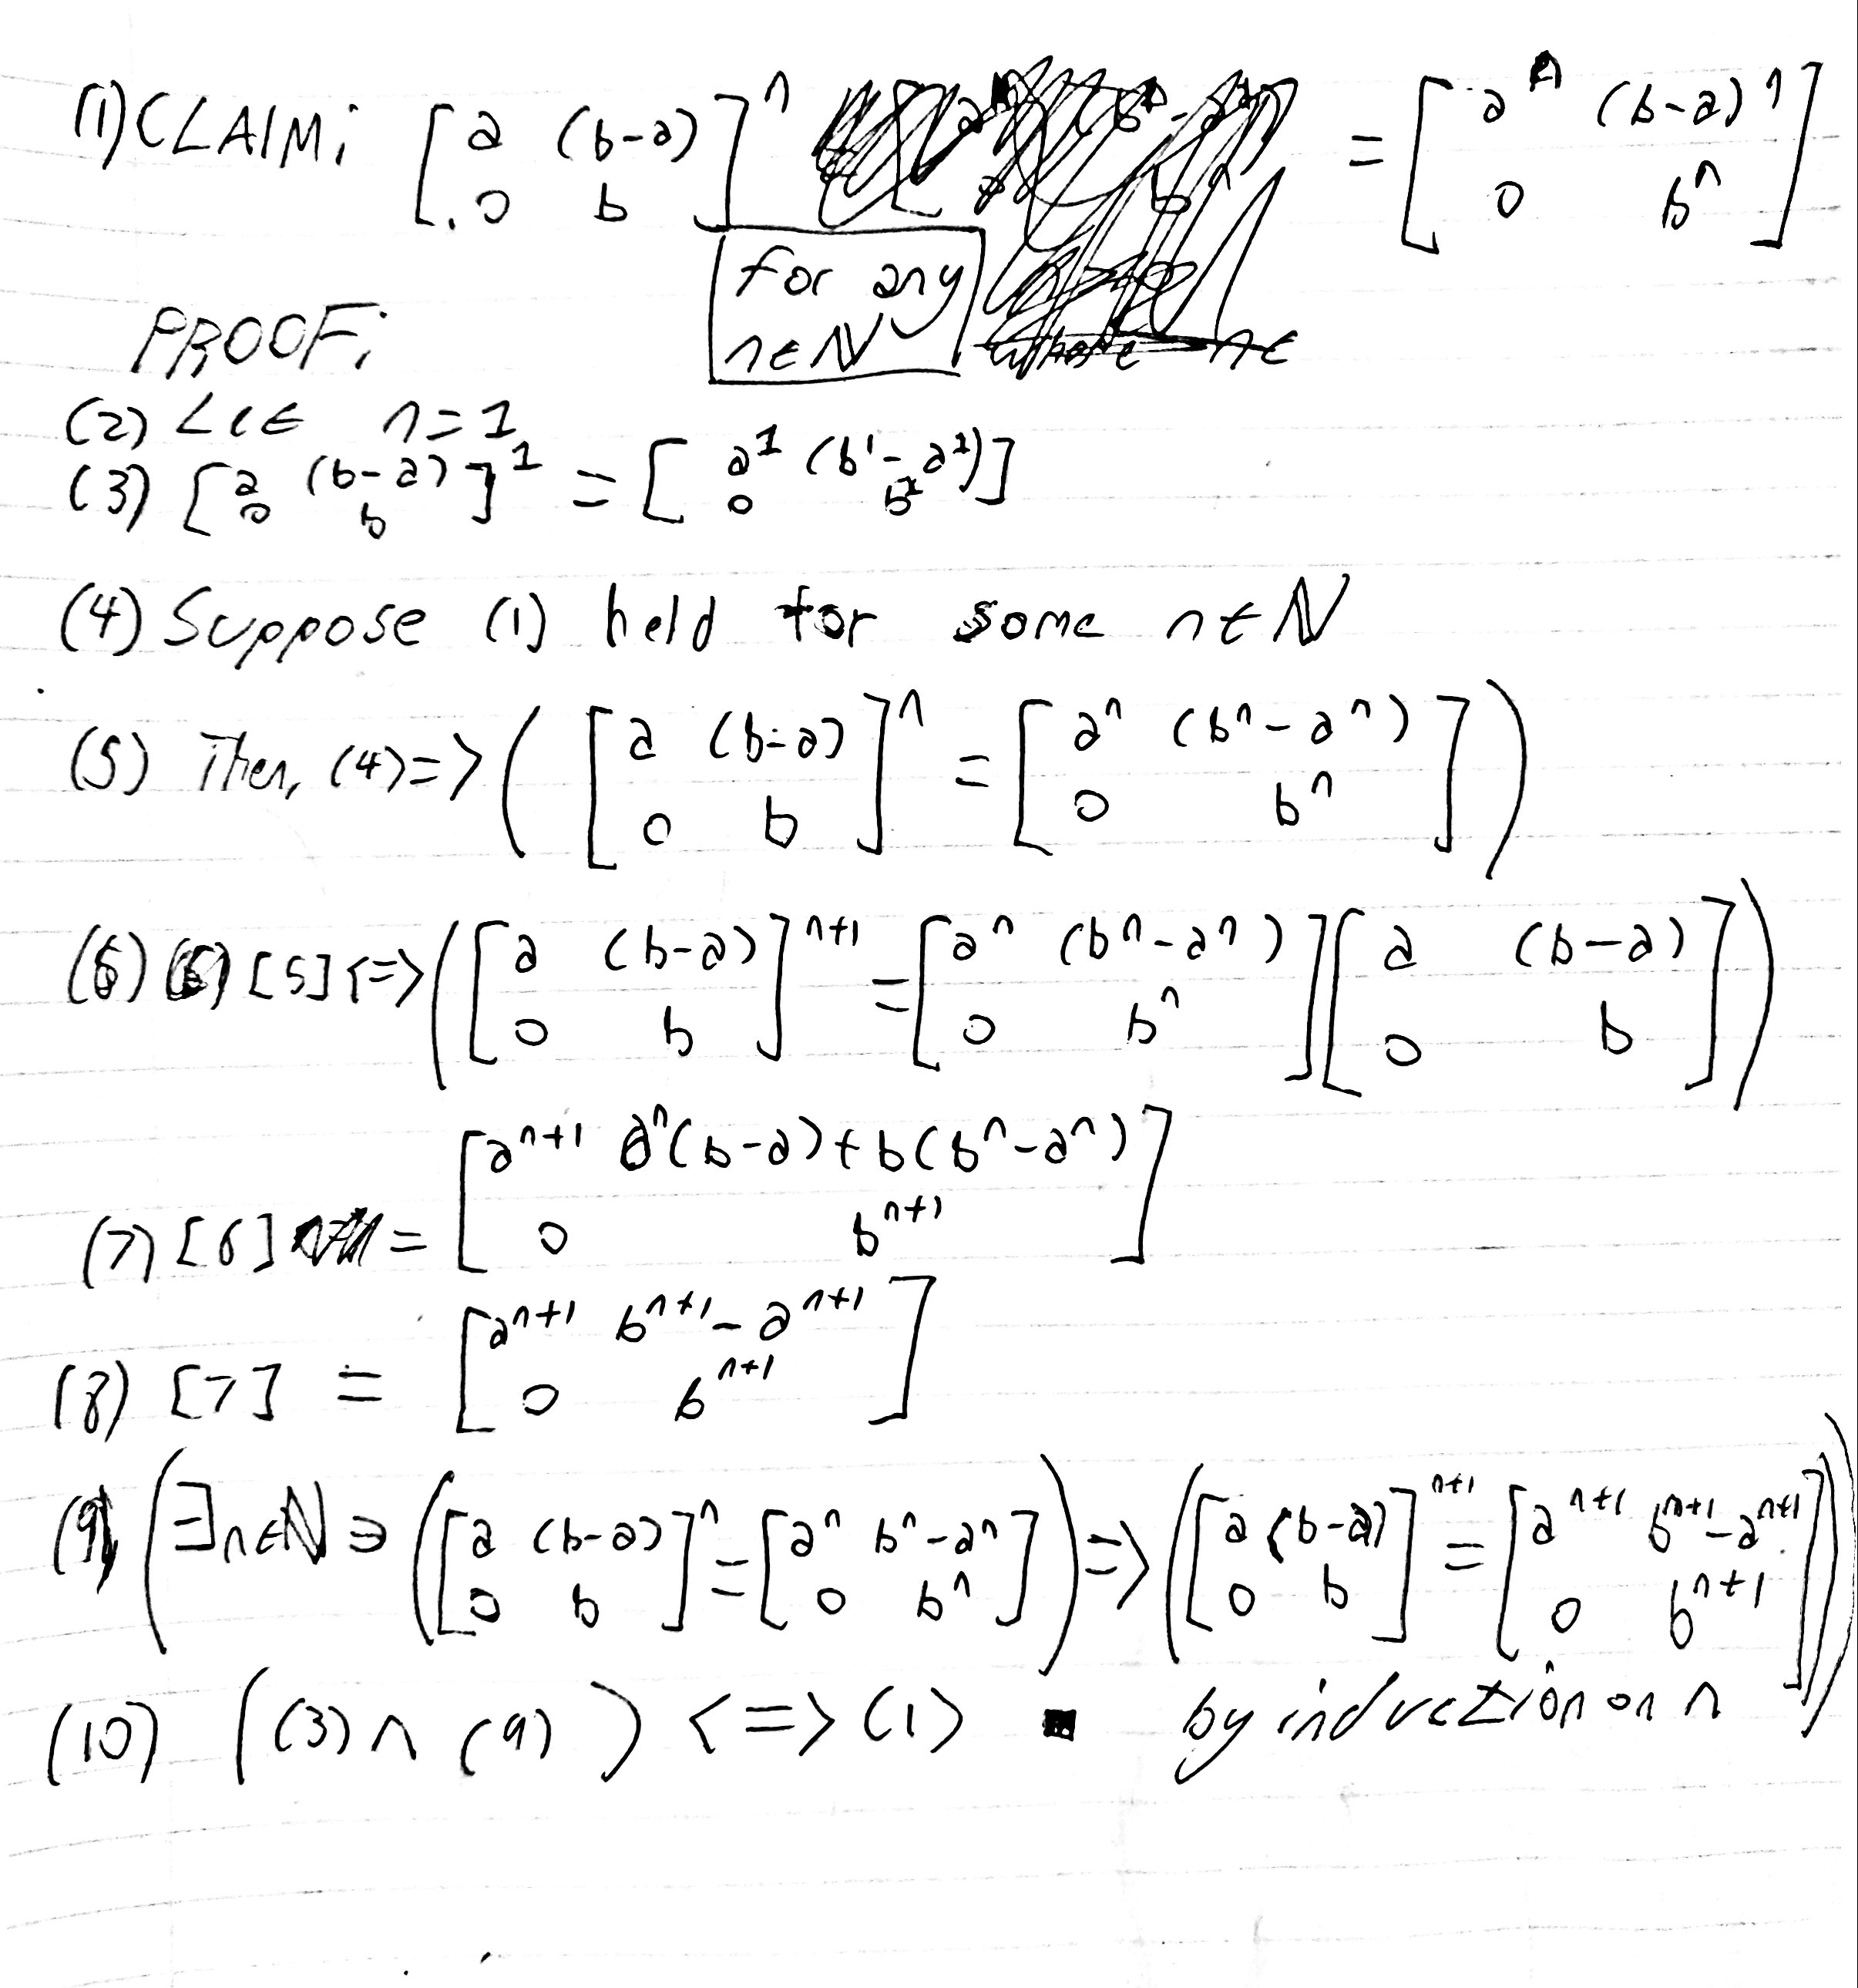
\includegraphics[scale=0.17]{proof12.jpg}
	\caption{An early sketch for the proof of theorem \ref{thm4}}
	\centering
	\label{proof12}
\end{figure}

\section{Proof of an equivalence relation}

Suppose $f,g,h \in \freals$.

Define the relation $\sim$ as:

\begin{align} \label{sim}
	f \sim g \iff \forall x \in \reals f(x) - g(x) = c \text{ for some } c \in \reals
\end{align}

\begin{thm} \label{thm5}
	$\sim$, as described in (\ref{sim}), is an equivalence relation
\end{thm}

\begin{proof}
	Obviously $f(x) - f(x) = 0 \in \reals$
	for all real $x$,
	so we have that $f \sim f$
	i.e. $\sim$ is reflexive.

	Then, if we suppose that $f(x) - g(x) = c \in \reals$
	for all real $x$,
	we must then have
	that $g(x) - f(x) = -c \in \reals$,
	so $f \sim g \implies g \sim f$
	i.e. $\sim$ is symmetric.

	Alternatively, if we suppose that both
	$f(x) - g(x) = c \in \reals \land g(x) - h(x) = d \in \reals$
	for all real $x$,
	we can add the two equations together to get
	$f(x) - h(x) = c + d \in \reals$,
	so we must have $f \sim g \land g \sim h \implies f \sim h$,
	i.e. $\sim$ is transitive.

	Finally, $\sim$ is
	reflexive,
	symmetric,
	and transitive
	if and only if
	$\sim$ is an equivalence relation.
	This proves theorem \ref{thm5}.
\end{proof}

\section{Proof of another equivalence relation}

Suppose $X$ is a set,
and define the bijection $f:X \to X$.

Define the following relation for some $a,b \in X$:
\begin{align} \label{sim2}
	a \sim b \iff \exists n \in \ints \ni f^n(a) = b
\end{align}

\begin{thm} \label{thm6}
	$\sim$, as described in (\ref{sim2}), is an equivalence relation
\end{thm}

\begin{proof}
	Suppose $a,b,c \in X$.

	Obviously $\exists n \in \ints \ni f^n(a) = a$
	since $f^0(a) = a$
	so we have that $a \sim a$
	i.e. $\sim$ is reflexive.

	Then, if we suppose that $a ~ b$,
	we have that some integer $n$ must
	exist such that $f^n(a) = b$,
	but since $f$ is bijective, we can apply $f^{-1}$
	to both sides of the last equation $n$ times
	to get $f^{-n}(b) = a$ and since $-n \in \ints$
	we then have $b \sim a$ and so
	we have the implication that
	$a \sim b \implies b \sim a$,
	i.e. $\sim$ is symmetric.

	Alternatively, if we suppose that
	$a \sim b \land b \sim c$ hold,
	we have integers $n$ and $m$ such that
	$f^n(a) = b \land f^m(b) = c$,
	so we can construct the composition
	$(f^n \circ f^m)(a) = f^{n + m}(a) = c$,
	and since $n + m \in \ints$,
	we have $a \sim c$ and so
	we have the implication that
	$a \sim b \land b \sim c \implies a \sim c$,
	i.e. $\sim$ is symmetric.

	Finally, $\sim$ is
	reflexive,
	symmetric,
	and transitive
	if and only if
	$\sim$ is an equivalence relation.
	This proves theorem \ref{thm6}.
\end{proof}

\end{document}
